%%%%%%%%%%%%%%%%%%%%%%%%%%%%%%%%%%%%%%%%%
% "ModernCV" CV and Cover Letter
% LaTeX Template
% Version 1.11 (19/6/14)
%
% Original template has been downloaded from:
% http://www.LaTeXTemplates.com
%
% Original author:
% Xavier Danaux (xdanaux@gmail.com)
%
% Modified by:
% WEN Hao (wenh06@gmail.com)
%
% License:
% CC BY-NC-SA 3.0 (http://creativecommons.org/licenses/by-nc-sa/3.0/)
%
% Important note:
% This template requires the moderncv.cls and .sty files to be in the same 
% directory as this .tex file. These files provide the resume style and themes 
% used for structuring the document.
%
%%%%%%%%%%%%%%%%%%%%%%%%%%%%%%%%%%%%%%%%%

%----------------------------------------------------------------------------------------
%	PACKAGES AND OTHER DOCUMENT CONFIGURATIONS
%----------------------------------------------------------------------------------------

\documentclass[10pt,a4paper,sans]{moderncv} % Font sizes: 10, 11, or 12; paper sizes: a4paper, letterpaper, a5paper, legalpaper, executivepaper or landscape; font families: sans or roman

\moderncvstyle{classic} % CV theme - options include: 'casual' (default), 'classic', 'oldstyle', 'fancy', and 'banking'

%-------------------------------------------------------
% definition of colors

%---------------------------------------------------------------------------------------
% built-in colors

\definecolor{black}{RGB}{0, 0, 0}
\definecolor{red}{rgb}{0.95, 0.20, 0.20}
\definecolor{darkgrey}{rgb}{0.45, 0.45, 0.45}
\definecolor{orange}{rgb}{0.95, 0.55, 0.15}
\definecolor{burgundy}{rgb}{0.596078, 0, 0}% 139/255 (0.545098) or 152/255 (0.596078)
\definecolor{purple}{rgb}{0.50, 0.33, 0.80}
\definecolor{lightblue}{rgb}{0.22, 0.45, 0.70}
\definecolor{green}{rgb}{0.35, 0.70, 0.30}

%---------------------------------------------------------------------------------------
% default colors

\colorlet{default-socialicon-color}{darkgrey}

%---------------------------------------------------------------------------------------
% custom colors

\definecolor{tsinghua}{rgb}{.434, .09, .531}
\definecolor{tsinghua-1}{HTML}{791CB5}
\definecolor{tsinghua-2}{HTML}{4B0C77}

%---------------------------------------------------------------------------------------
% colors for social icons

\definecolor{weixin}{rgb}{.184, .533, .098}
\definecolor{linkedin}{HTML}{0a66c2}
\definecolor{orcid}{HTML}{a6ce39}
\definecolor{twitter}{RGB}{29, 155, 240}
\definecolor{facebook}{HTML}{1b74e4}

\colorlet{address}{tsinghua-1}
\colorlet{mobilephone}{tsinghua-1}
\colorlet{fixedphone}{tsinghua-1}
\colorlet{faxphone}{tsinghua-1}
\colorlet{email}{tsinghua-1}
\colorlet{homepage}{tsinghua-1}
\colorlet{googlescholar}{tsinghua-1}


%-------------------------------------------------------

\moderncvcolor{tsinghua-1} % CV color - options include: 'tsinghua', 'blue' (default), 'orange', 'green', 'red', 'purple', 'grey' and 'black'

% \usepackage{lipsum} % Used for inserting dummy 'Lorem ipsum' text into the template

\usepackage[scale=.88]{geometry} % Reduce document margins
%\setlength{\hintscolumnwidth}{3cm} % Uncomment to change the width of the dates column
%\setlength{\makecvtitlenamewidth}{10cm} % For the 'classic' style, uncomment to adjust the width of the space allocated to your name
% \usepackage{hyperref}
\usepackage{tikz}
\usetikzlibrary{calc}
\usepackage{graphicx}

\moderncvicons{academic}


%-------------------------------------------------------
% bib settings


% \usepackage[style=authoryear,sorting=ydnt,dashed=false,maxbibnames=99]{biblatex}

% \renewbibmacro*{date}{}
% \renewbibmacro*{date+extrayear}{}
% \renewbibmacro*{issue+date}{}
% \newcommand*{\bibyear}{}

% \defbibenvironment{bibliography}
% {\list
%  {\iffieldequals{year}{\bibyear}
%     {}
%     {\printfield{year}%
%      \savefield{year}{\bibyear}}}
%  {\setlength{\topsep}{0pt}% layout parameters based on moderncvstyleclassic.sty
%   \setlength{\labelwidth}{\hintscolumnwidth}%
%   \setlength{\labelsep}{\separatorcolumnwidth}%
%   \setlength{\itemsep}{\bibitemsep}%
%   \leftmargin\labelwidth%
%   \advance\leftmargin\labelsep}%
%   \sloppy\clubpenalty4000\widowpenalty4000}
% {\endlist}
% {\item}

% \addbibresource{publications.bib}

\usepackage{moderntimeline}
\tlmaxdates{2016}{2023}

\newif\ifnumericCVbibliography
\numericCVbibliographytrue % replace true with false to disable
\newlength{\hintscolumnwidthV}
\setlength\hintscolumnwidthV{\hintscolumnwidth}
\newlength{\labelkern}
\ifnumericCVbibliography
  \setlength\labelkern{-2ex}
  \usepackage[backend = biber,
              style   = nature,
              sorting=ydnt
             ]{biblatex}
  \newcommand{\printbibnumber}{%\hspace* here has no effect so I removed it
      \llap{\printtext[labelnumberwidth]{%
              \printfield{labelprefix}%
              \printfield{labelnumber}
              }\kern\labelkern% to reduce space between label and timeline image
            }%
  }
\else
  \usepackage[backend = biber,
              style   = authoryear,
              sorting=ydnt
             ]{biblatex}
  \newcommand{\printbibnumber}{\relax} % do nothing
  \setlength\labelkern{0ex}
  \setlength\hintscolumnwidthV{\hintscolumnwidth} % this length needs 
  % to be re-set or it keeps the numeric  version value if that has been run before
\fi
\addbibresource{publications.bib}
%-----------------------------------------------------------
\makeatletter
\newcommand*{\cventryV}[1][.25em]{}
% timeline for bibliography
\newcommand{\tldatecventryV}[2][color1]{%
\issincefalse
\tl@formatstartyear{#2}
\cventryV{\tikz[baseline=0pt]{
    \useasboundingbox (0ex,0ex) rectangle (\hintscolumnwidthV,1ex); 
    %changed origin of boundingbox. previous was (2ex,0ex) but this 
    % creates alignment problems when switching between numeric and non numeric.
    \fill [\tl@runningcolor] (0,0)
       rectangle (\hintscolumnwidthV,\tl@runningwidth);
    \fill [#1] (0,0)
       ++(\tl@startfraction*\hintscolumnwidthV,0pt)
       node [tl@singleyear] {#2}
       node {$\bullet$};
  }}}
\makeatother
%-----------------------------------
\defbibenvironment{bibliography}
  {\list
   {\printbibnumber% here you see the macro in action
    \tldatecventryV{%
      \thefield{year} % actual year from bibitem
       }}
       {%
        \setlength{\topsep}{0pt}% layout parameters based on moderncvstyleclassic.sty
        \addtolength\hintscolumnwidthV{-\labelnumberwidth}% num - changes timeline image length
        \addtolength\hintscolumnwidthV{\labelkern}% num  - changes timeline image length
        \setlength{\bibhang}{\hintscolumnwidthV} % custom bibhang
        \setlength{\labelsep}{\separatorcolumnwidth} %  horizontal distance between label and entry
        \setlength{\leftmargin}{\hintscolumnwidth} % sets where the left margin is
        \addtolength{\leftmargin}{\separatorcolumnwidth} %
        \setlength{\itemindent}{-\bibhang} % this sets indentation of the second line of the entry.
        % changing it moves also the first line left or right
        \addtolength{\itemindent}{-\separatorcolumnwidth} % to align the second line exactly
        \setlength{\itemsep}{\bibitemsep} % vertical distance between bib items
        \setlength{\parsep}{\bibparsep}}}
  {\endlist}
  {\item}
%-----------------------
\AtEveryBibitem{\clearfield{year}}
%-------------------------------------------------------------------------------
%  reverse numbering of publications
%-------------------------------------------------------------------------------
% Count total number of entries in each refsection
\AtDataInput{%
  \csnumgdef{entrycount:\therefsection}{%
    \csuse{entrycount:\therefsection}+1}}
% Print the labelnumber as the total number of entries in the
% current refsection, minus the actual labelnumber, plus one
\DeclareFieldFormat{labelnumber}{\mkbibdesc{#1}}
\newrobustcmd*{\mkbibdesc}[1]{%
  \number\numexpr\csuse{entrycount:\therefsection}+1-#1\relax}


%-------------------------------------------------------


%-------------------------------------------------------
% new commands

\newcommand{\cvdoublecolumn}[2]{
  \cvitem[0.75em]{}{
    \begin{minipage}[t]{\listdoubleitemcolumnwidth}#1\end{minipage}
    \hfill
    \begin{minipage}[t]{\listdoubleitemcolumnwidth}#2\end{minipage}
  }
}

\newcommand{\cvreference}[9]{
  \textbf{#1}\newline % Name
  \ifthenelse{\equal{#2}{}}{}{\addresssymbol~#2\newline} % address
  \ifthenelse{\equal{#3}{}}{}{#3\newline} % department
  \ifthenelse{\equal{#4}{}}{}{#4\newline} % affiliation
  \ifthenelse{\equal{#5}{}}{}{#5\newline} % city, country
  \ifthenelse{\equal{#6}{}}{}{\homepagesymbol~#6\newline} % homepage
  \ifthenelse{\equal{#7}{}}{}{\emailsymbol~\texttt{\href{mailto:#7}{\nolinkurl{#7}}} \newline} % email
  \ifthenelse{\equal{#8}{}}{}{\fixedphonesymbol~#8\newline} % fixed phone
  \ifthenelse{\equal{#9}{}}{}{\mobilephonesymbol~#9} % mobile phone
}


%-------------------------------------------------------


%-------------------------------------------------------
% switches

%--------------------------------------------------------------------
% whether to include the education section
%--------------------------------------------------------------------
\newif\ifEducationSection
\EducationSectiontrue

%--------------------------------------------------------------------
% whether to include high school in the education section
%--------------------------------------------------------------------
\newif\ifHighSchool
\HighSchoolfalse

%--------------------------------------------------------------------
% whether to include the awards section
%--------------------------------------------------------------------
\newif\ifAwardsSection
\AwardsSectionfalse

%--------------------------------------------------------------------
% whether to include the research interest section
%--------------------------------------------------------------------
\newif\ifResearchInterestSection
\ResearchInterestSectiontrue

%--------------------------------------------------------------------
% whether to include the research experience section
%--------------------------------------------------------------------
\newif\ifResearchExperienceSection
\ResearchExperienceSectiontrue

%--------------------------------------------------------------------
% whether to include the work experience section
%--------------------------------------------------------------------
\newif\ifWorkExperienceSection
\WorkExperienceSectiontrue

%--------------------------------------------------------------------
% whether to include the publications section
%--------------------------------------------------------------------
\newif\ifPublicationsSection
\PublicationsSectiontrue

%--------------------------------------------------------------------
% whether to include the PhD thesis section
%--------------------------------------------------------------------
\newif\ifPhdThesisSection
\PhdThesisSectionfalse

%--------------------------------------------------------------------
% whether to include the invited talks section
%--------------------------------------------------------------------
\newif\ifInvitedTalksSection
\InvitedTalksSectiontrue

%--------------------------------------------------------------------
% whether to include the teaching section
%--------------------------------------------------------------------
\newif\ifTeachingSection
\TeachingSectiontrue

%--------------------------------------------------------------------
% whether to include miscellaneous section
%--------------------------------------------------------------------
\newif\ifMiscSection
\MiscSectionfalse

%--------------------------------------------------------------------
% whether to include the language section
%--------------------------------------------------------------------
\newif\ifLanguageSection
\LanguageSectiontrue

%--------------------------------------------------------------------
% whether to include the Skills and Open source community section
%--------------------------------------------------------------------
\newif\ifSkillsAndOscSection
\SkillsAndOscSectiontrue

%--------------------------------------------------------------------
% whether to include the interests section
%--------------------------------------------------------------------
\newif\ifInterestsSection
\InterestsSectionfalse

%--------------------------------------------------------------------
% whether to include the list of references
%--------------------------------------------------------------------
\newif\ifListReferences
\ListReferencesfalse

%--------------------------------------------------------------------
% whether to include the cover letter
%--------------------------------------------------------------------
\newif\ifCoverLetter
\CoverLetterfalse

%--------------------------------------------------------------------
% whether to include teaching statement
%--------------------------------------------------------------------
\newif\ifTeachingStatement
\TeachingStatementfalse

%--------------------------------------------------------------------
% whether to include research statement
%--------------------------------------------------------------------
\newif\ifResearchStatement
\ResearchStatementfalse


\ifdefined\ifChinese
% pass
\else
\newif\ifChinese
\fi

% \Chinesetrue
\HighSchoolfalse

% more switches can be found in commons/switches.tex
% \EducationSectiontrue
% \AwardsSectionfalse
% \ResearchInterestSectiontrue
% \ResearchExperienceSectiontrue
% \WorkExperienceSectiontrue
% \PublicationsSectiontrue
% \PhdThesisSectionfalse
% \InvitedTalksSectiontrue
% \TeachingSectiontrue
% \MiscSectionfalse
% \LanguageSectiontrue
% \SkillsAndOscSectiontrue
% \InterestsSectionfalse
% \ListReferencesfalse
% \CoverLetterfalse
% \TeachingStatementfalse
% \ResearchStatementfalse

%-------------------------------------------------------


%-------------------------------------------------------
% heading

% requires load commons/switches before loading this file

\ifChinese

\usepackage[T1]{fontenc}
\usepackage[BoldFont,SlantFont]{xeCJK}
% \setCJKmainfont[Path = fonts/, BoldFont = simhei.ttf]{simfang.ttf}
% \setCJKsansfont[Path = fonts/]{simhei.ttf}
% \setCJKmonofont[Path = fonts/]{simkai.ttf}
\setCJKmainfont{Noto Serif CJK SC}
\setCJKsansfont{Noto Sans CJK SC}
\setCJKmonofont{Noto Sans Mono CJK SC}


%----------------------------------------------------------------------------------------
%	NAME AND CONTACT INFORMATION SECTION
%----------------------------------------------------------------------------------------

\firstname{文豪} % Your first name
\familyname{ } % Your last name

% \renewcommand*{\refname}{发表文章}


% All information in this block is optional, comment out any lines you don't need
\title{个人简历}
% \address{近春园西楼数学中心 309,}{北京, 清华大学, 100084}
\address{北京航空航天大学}{沙河校区E301}

%----------------------------------------------------------------------------------------
% socials


\mobile{(+86) 15901026741}
\email{wenh06@gmail.com}
% \homepage{https://www.linkedin.com} {https://www.linkedin.com} % The first argument is the url for the clickable link, the second argument is the url displayed in the template - this allows special characters to be displayed such as the tilde in this example
\social[orcid][orcid.org/0000-0002-8856-0883]{0000-0002-8856-0883}
\social[googlescholar][scholar.google.com/citations?user=AdRRAw0AAAAJ\&hl=en]{Google Scholar {[Hao Wen]}}
\social[wos][www.webofscience.com/wos/author/record/AAC-8935-2022]{WOS ResearcherID: AAC-8935-2022}
\social[github][github.com/wenh06]{https://github.com/wenh06}
\social[pypi][pypi.org/user/wenh06]{https://pypi.org/user/wenh06}
\social[linkedin][www.linkedin.com/in/wenh06]{wenh06}


%----------------------------------------------------------------------------------------

\extrainfo{
{\color{weixin}\faWeixin} wen2010310927 \\{\color{tsinghua}性别} 男 {\color{tsinghua}|} {\color{tsinghua}出生日期} 1987.12.16
}
\photo[92pt][0.4pt]{images/bachelor} % The first bracket is the picture height, the second is the thickness of the frame around the picture (0pt for no frame)
%\quote{"A witty and playful quotation" - John Smith}
%----------------------------------------------------------------------------------------


\else  % else of \ifChinese


%----------------------------------------------------------------------------------------
%	NAME AND CONTACT INFORMATION SECTION
%----------------------------------------------------------------------------------------

\firstname{Hao} % Your first name
\familyname{WEN} % Your last name


% All information in this block is optional, comment out any lines you don't need
\title{Curriculum Vitae}
\address{E301, Shahe Campus}{Beihang University}

%----------------------------------------------------------------------------------------
% socials


\mobile{(+86) 15901026741}
\email{wenh06@gmail.com}
% \homepage{https://www.linkedin.com} {https://www.linkedin.com} % The first argument is the url for the clickable link, the second argument is the url displayed in the template - this allows special characters to be displayed such as the tilde in this example
\social[orcid][orcid.org/0000-0002-8856-0883]{0000-0002-8856-0883}
\social[googlescholar][scholar.google.com/citations?user=AdRRAw0AAAAJ\&hl=en]{Google Scholar {[Hao Wen]}}
\social[wos][www.webofscience.com/wos/author/record/AAC-8935-2022]{WOS ResearcherID: AAC-8935-2022}
\social[github][github.com/wenh06]{https://github.com/wenh06}
\social[pypi][pypi.org/user/wenh06]{https://pypi.org/user/wenh06}
\social[linkedin][www.linkedin.com/in/wenh06]{wenh06}


%----------------------------------------------------------------------------------------

\extrainfo{
{\color{weixin}\faWeixin} wen2010310927 \\{\color{tsinghua}Gender} Male {\color{tsinghua}|} {\color{tsinghua}Born} 1987.12.16
}
\photo[87pt][0.4pt]{images/bachelor} % The first bracket is the picture height, the second is the thickness of the frame around the picture (0pt for no frame)
%\quote{"A witty and playful quotation" - John Smith}
%----------------------------------------------------------------------------------------

\fi  % fi of \ifChinese


%-------------------------------------------------------


\begin{document}

%-------------------------------------------------------
% contents

%----------------------------------------------------------------------------------------
%	Headings
%----------------------------------------------------------------------------------------

% wechat QRcode
\begin{tikzpicture}[overlay, remember picture]
\node[anchor=north west, %anchor is upper left corner of the graphic
      xshift=1.2cm, %shifting around
      yshift=-1.5cm]
     at (current page.north west) %left upper corner of the page
     {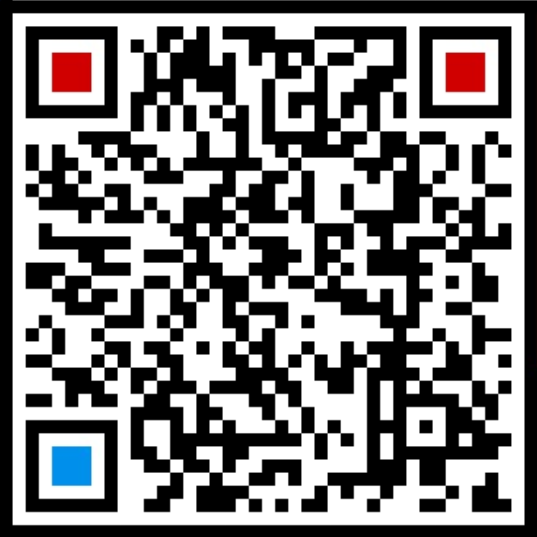
\includegraphics[width=2.2cm]{images/wx_qrcode.png}}; 
\end{tikzpicture}


\makecvtitle % Print the CV title

%----------------------------------------------------------------------------------------
%	EDUCATION SECTION
%----------------------------------------------------------------------------------------

\ifEducationSection

\ifChinese

\section{教育背景}

\cventry{2010.9--2018.1}{清华大学}{}{}{}{\normalsize 理学博士,数学}

\cventry{2006.8--2010.6}{清华大学}{}{}{}{\normalsize 理学学士,数学物理基础科学班}

\ifHighSchool
\cventry{2002.9--2006.6}{萍乡中学}{}{}{}{}
\fi

\else  % else of \ifChinese

\section{Education}

\cventry{2010.9--2018.1}{Tsinghua University}{}{}{}{\normalsize {\bfseries Doctor} of Philosophy, \textit{Mathematics}}

\cventry{2006.8--2010.6}{Tsinghua University}{}{}{}{\normalsize {\bfseries Bachelor} of Science, \textit{Mathematics and Physics}}

\fi  % fi of \ifChinese

\fi  % fi of \ifEducationSection


%----------------------------------------------------------------------------------------
%	AWARDS SECTION
%----------------------------------------------------------------------------------------

\ifAwardsSection

\ifChinese

\section{获得奖励}

% \cventry{April 2015 --
% April 2017}{Certified LabVIEW Associate Developer}{\textsc{National Instruments}}{}{}{}

\else  % else of \ifChinese

\section{Certifications}

% \cventry{April 2015 --
% April 2017}{Certified LabVIEW Associate Developer}{\textsc{National Instruments}}{}{}{}

\fi  % fi of \ifChinese

\fi  % fi of \ifAwardsSection


%----------------------------------------------------------------------------------------
%	RESEARCH INTEREST SECTION
%----------------------------------------------------------------------------------------

\ifResearchInterestSection

\ifChinese

\section{研究领域}

\cvitem{}{
\textbf{机器学习,深度学习,最优化理论与应用}
\newline
数论,代数几何,表示论 ,密码学,模式识别,信号处理
}

\else  % else of \ifChinese

\section{Research Interests}

\cvitem{}{\textbf{Federated Learning, Deep Learning, Mathematical Optimization} - Theory and Applications
\newline
Number Theory, Arithmetic Geometry, Representation Theory, Cryptography, Pattern Recognition
}

\fi  % fi of \ifChinese

\fi  % fi of \ifResearchInterestSection


%----------------------------------------------------------------------------------------
%	RESEARCH EXPERIENCE SECTION
%----------------------------------------------------------------------------------------

\ifResearchExperienceSection

\ifChinese

\section{研究经历}

\cventry{2021.3
至今}{Federated Learning, Large-Scale Non-Convex Optimization}{\newline 合作导师:韩德仁教授}{北京航空航天大学}{}{}

\cventry{2019.1 --
2021.1}{Cognitive Computing for Precision Health}{\newline 合作导师:喻文健副教授,吴元清博士}{清华大学,京东健康医疗创新研发部}{}{}

\cventry{2017.3 --
2018.1}{Counting Multiplicities in a Hypersurface over Number Fields}{\newline 合作者:刘春晖博士}{Universit\'{e} Paris Diderot,法国}{}{}

\cventry{2016.5 --
2017.3}{Characters of the General Linear Supergroups}{\newline 指导教师:张贺春教授}{清华大学}{}{}

\cventry{2014.1 --
2015.6}{Computation of Modular Units}{\newline 指导教师:印林生教授}{清华大学}{}{}

\cventry{2013.1 --
2013.7}{N\'{e}ron Models of Semi-Abelian Varieties}{\newline 访问学者}{\emph{指导教师:刘青教授}}{Universit\'{e} Bordeaux 1,法国}{}

\cventry{2012.1 --
2013.12}{Galois Representation and Modular Forms}{\newline 指导教师:印林生教授}{清华大学}{}{}

\cventry{2011.1 --
2012.12}{Elliptic-Curve Cryptography}{\newline 指导教师:印林生教授}{清华大学}{}{}

\else  % else of \ifChinese

\section{Research Experience}

\cventry{Jan. 2021 -- Current}{Federated Learning, Large-Scale Non-Convex Optimization}{\newline School of Mathematical Sciences}{Beihang University}{}{}

\cventry{Jan. 2019 -- Jan. 2021}{Cognitive Computing for Precision Health}{\newline Department of Computer Science and Technology}{Tsinghua University}{}{}

\cventry{Mar. 2017 -- Jan. 2018}{Counting Multiplicities in a Hypersurface over Number Fields}{\newline Co-author with Dr. Chunhui Liu}{Universit\'{e} Paris Diderot}{}{}

\cventry{May 2016 -- Mar. 2017}{Characters of the General Linear Supergroups}{\newline Research team of Prof. Hechun Zhang}{Department of Mathematical Sciences}{Tsinghua University}{}

\cventry{Jan. 2014 -- June 2015}{Computation of Modular Units}{\newline Research team of Prof. Linsheng Yin}{Department of Mathematical Sciences}{Tsinghua University}{}

\cventry{Jan. 2013 -- June 2013}{N\'{e}ron Models of Semi-Abelian Varieties}{\newline Visiting Scholar}{Universit\'{e} Bordeaux 1}{France}{}

\cventry{Jan. 2012 -- Dec. 2013}{Galois Representation and Modular Forms}{\newline Research team of Prof. Linsheng Yin}{Department of Mathematical Sciences}{Tsinghua University}{}

\cventry{Jan. 2011 -- Dec. 2012}{Elliptic-Curve Cryptography}{\newline Research team of Prof. Linsheng Yin}{Tsinghua University}{}{}

\fi  % fi of \ifChinese

\fi  % fi of \ifResearchExperienceSection


%----------------------------------------------------------------------------------------
%	WORK EXPERIENCE SECTION
%----------------------------------------------------------------------------------------

\ifWorkExperienceSection

\ifChinese

\section{创业与工作经历}

\cventry{2021.3 至今}{北京航空航天大学博士后}{}{}{}{联邦学习中的优化算法以及在医疗中的应用;深度学习在医学图像、信号处理中的应用。}

\cventry{2018.10 --
2021.1}{京东健康医疗创新研发部算法工程师、企业博士后}{}{}{}{采用传统信号处理,模式识别,结合机器学习深度学习等多种工具,与京东健康医疗创新研发部同事合作,分别搭建了3个完整的智慧医疗系统,包括连续血糖监护分析平台,心电监护分析平台,以及中医望诊平台。}

\cventry{2014.10 --
2016.9}{与别人合伙创立\textsc{Houyi Tech., Inc.},并担任兼职算法开发人员}{}{}{}{采用小面积传感器在嵌入式的 ARM STM32 嵌入式芯片上实现了指纹认证系统(软件著作权登记号2015SR079424),并在消费电子以及公证处等多个场景落地。}

\else  % else of \ifChinese

\section{Entrepreneurial and Work Experience}

\cventry{2021.3 --
Current}{\textsc{Beihang University}}{Postdoctoral Fellow}{}{}{Optimization algorithms in Federated Learning and applications in Healthcare; Applications of deep learning in medical image and signal processing.}

\cventry{2018.10 --
2021.1}{\textsc{JD Health International Inc.}}{Algorithm Engineer and Corporate Postdoctoral Fellow}{}{}{Pattern recognition, machine learning and deep learning for medical image and signal processing; Design and implement smart medical systems: continuous blood glucose monitoring and analysis platform, ECG monitoring analysis platform, the TCM observation and diagnosis platform.}

\cventry{2014.10 --
2016.9}{\textsc{Houyi Tech. Inc.}}{Co-founder and Algorithm Engineer}{}{}{Embedded Implementation of Fingerprint Recognition Systems on ARM STM32 platforms.}

\fi  % fi of \ifChinese

\fi  % fi of \ifWorkExperienceSection


%----------------------------------------------------------------------------------------
%	PUBLICATIONS SECTION
%----------------------------------------------------------------------------------------

\ifPublicationsSection

\ifChinese

\nocite{phdthesis-zh,wen_liu,Kang_2022_cinc2021_iop,torch_ecg_paper,Wen_cpsc2021,wen_cinc2021,qi2021kemre,af_detection,acne_detection}
\printbibliography[title={发表文章}]

\else  % else of \ifChinese

\nocite{phdthesis-en,wen_liu,Kang_2022_cinc2021_iop,torch_ecg_paper,Wen_cpsc2021,wen_cinc2021,qi2021kemre,af_detection,acne_detection}
\printbibliography[title={Publications}]

\fi  % fi of \ifChinese

\fi  % fi of \ifPublicationsSection


%----------------------------------------------------------------------------------------
%	Ph.D. SECTION
%----------------------------------------------------------------------------------------

\ifPhdThesisSection

\ifChinese

\section{博士论文}

\cvitem{题目}{\bfseries 定义在数域上的超曲面的重数计数问题}
\cvitem{导师}{{\bfseries 张贺春} 教授}
\cvitem{评审人}{唐舜,徐飞(首都师范大学),\newline
王崧(中国科学院晨兴数学中心),\newline
姚家燕(清华大学)}
\cvitem{答辩委员会}{徐飞({\bfseries 主席},首都师范大学),\newline
郑维喆(中国科学院晨兴数学中心),\newline
姚家燕,朱斌,邓邦明(清华大学)}
\cvitem{论文简介}{考虑定义在数域上的射影超曲面,可以通过局部 Hilbert-Samuel 函数定义其上点的重数。取定一个计数函数,考虑在这个射影超曲面上代数点的重数的计数问题:即对超曲面上,高度不超过定值,定义域相对于基域的扩张次数等于一个定值的所有代数点,用取定的计数函数作用在这些点的重数上,求和。论文对这个问题给出了一个上界估计,这个上界将会与射影超曲面的次数,奇点集的维数,高度的上界,以及相应域扩张次数有关。这个估计可以在某种程度上衡量射影超曲面的奇点集的复杂程度。}

\else  % else of \ifChinese

\section{Ph.D. Thesis}

\cvitem{Title}{\emph{Counting Multiplicities in a Hypersurface over Number Fields}}
\cvitem{Supervisor}{Professor {\bfseries Hechun ZHANG}}
\cvitem{Reviewers}{Shun TANG, Fei XU (Capital Normal University),\newline Song WANG (Chinese Academy of Sciences),\newline Jiayan YAO (Tsinghua University)}
\cvitem{Committee Members}{Fei XU ({\bfseries Chair}, Capital Normal University),\newline Weizhe ZHENG (Chinese Academy of Sciences),\newline Jiayan YAO, Bin ZHU, Bangming DENG (Tsinghua University)}
\cvitem{Description}{Fix a counting function of multiplicities of algebraic points in a projective hypersurface over a number field, and take the sum over all algebraic points of bounded height and fixed degree. An upper bound for the sum with respect to this counting function is given in terms of the degree of the hypersurface, the dimension of the singular locus, the upper bounds of height, and the degree of the field of definition. This upper bound describes the complexity of this hypersurface's singular locus to some extent.}

\fi  % fi of \ifChinese

\fi  % fi of \ifPhdThesisSection


%----------------------------------------------------------------------------------------
%	INVITED TALKS SECTION
%----------------------------------------------------------------------------------------

\ifInvitedTalksSection

\ifChinese

\section{受邀报告}

\cventry{2022.9}{The 49th Computing in Cardiology Conference}{\newline \textsc{题目:Searching for Effective Neural Network Architectures for Heart Murmur Detection from Phonocardiogram}}{\newline Poster}{Online (offline at Tampere, Finland)}{}

\cventry{2021.11}{The 10th International Conference on Biomedical Engineering and Biotechnology (ICBEB 2021)}{\newline \textsc{题目:Accurate Paroxysmal Atrial Fibrillation Events
Detection using Deep Neural Networks}}{\newline Oral}{Online}{}

\cventry{2021.9}{The 48th Computing in Cardiology Conference}{\newline \textsc{题目:Hybrid Arrhythmia Detection on Varying-Dimensional ECG: Combining Deep Neural Networks and Clinical Rules}}{\newline Poster}{Online (offline at Brno, Czech Republic)}{}

\cventry{2017.9}{Intercity Seminar on Arakelov Theory, the 2017 Session in Beijing}{\newline \textsc{题目:Counting Multiplicities in a Hypersurface over Number Fields}}{\newline 首都师范大学}{北京}{}

\cventry{2017.4}{清华大学博士生论坛}{\newline \textsc{题目:Characters of the General Linear Supergroups}}{\newline 三堡学术基地}{北京}{}

\else  % else of \ifChinese

\section{Invited Talks}

\cventry{2022.9}{The 49th Computing in Cardiology Conference}{\newline \textsc{Title: Searching for Effective Neural Network Architectures for Heart Murmur Detection from Phonocardiogram}}{\newline Poster}{Online (offline at Tampere, Finland)}{}

\cventry{Nov. 2021}{The 10th International Conference on Biomedical Engineering and Biotechnology (ICBEB 2021)}{\newline \textsc{Title: Accurate Paroxysmal Atrial Fibrillation Events
Detection using Deep Neural Networks}}{\newline Oral}{Online}{}

\cventry{Sept. 2021}{The 48th Computing in Cardiology Conference}{\newline \textsc{Title: Hybrid Arrhythmia Detection on Varying-Dimensional ECG: Combining Deep Neural Networks and Clinical Rules}}{\newline Poster}{Online (offline at Brno, Czech Republic)}{}

\cventry{Sept. 2017}{Intercity Seminar on Arakelov Theory, the 2017 Session in Beijing}{\newline \textsc{Title: Counting Multiplicities in a Hypersurface over Number Fields}}{\newline Capital Normal University}{Beijing}{}

\cventry{Apr. 2017}{Forum of Ph.D. Candidates organised by Tsinghua University}{\newline \textsc{Title: Characters of the General Linear Supergroups}}{\newline Sanbao Academic Base}{Beijing}{}

\fi  % fi of \ifChinese

\fi  % fi of \ifInvitedTalksSection


%----------------------------------------------------------------------------------------
% TEACHING EXPERIENCE SECTION
%----------------------------------------------------------------------------------------

\ifTeachingSection

\renewcommand{\listitemsymbol}{-~} % Changes the symbol used for lists

\ifChinese

\section{助教工作}

\cvlistdoubleitem{高等代数}{微积分}
\cvlistdoubleitem{代数数论}{抽象代数}
% \cvlistdoubleitem{高等代数与几何}{}

\else  % else of \ifChinese

\section{Teaching Assistant}

\cvlistdoubleitem{Calculus}{Advanced Calculus}
\cvlistdoubleitem{Linear Algebra}{Advanced Algebra}
\cvlistdoubleitem{Algebraic Number Theory}{Abstract Algebra}
% \cvlistdoubleitem{Advanced Algebra and Geometry}{}

\fi  % fi of \ifChinese

\fi  % fi of \ifTeachingSection


%----------------------------------------------------------------------------------------
% Miscellaneous SECTION
%----------------------------------------------------------------------------------------

\ifMiscSection

\ifChinese

\section{其他经历}

\cventry{Jul. 2012 --
Aug. 2012}{Dongfang Electric Corporation}{}{Guangzhou}{}{Research and technological development of information security of the enterprise.}

\cventry{2020.11}{3rd China Physiological Signal Challenge 2020 (CPSC2020) 竞赛项目 SPBerr 第三名}{}{}{}{}{}

\cventry{2014.9 --
2015.12}{课程助教}{\href{http://www.xuetangx.com/}{学堂在线}}{}{}{作为清华大学数学系马辉教授所教授的《线性代数1》与《线性代数2》的学堂在线MOOC课程的助教,协助其制作PPT课件,并维护课程论坛。}

\cventry{2014.8 --
2014.10}{China-Korea Joint Seminar on Number Theory}{}{海南三亚}{}{协助印林生教授组织会议。}

\cventry{2014.10 --
2015.12}{兼职算法开发人员}{\textsc{Houyi Tech., Inc.}}{}{}{与别人合作,在 ARM STM32 嵌入式芯片上实现了指纹识别等功能(软件著作权登记号2015SR079424),并在多个应用场景落地。}

\else  % else of \ifChinese

\section{Miscellaneous}

\cventry{Nov. 2020}{3rd place in SPBerr in the 3rd China Physiological Signal Challenge 2020 (CPSC2020)}{}{}{}{}{}

\cventry{Jul. 2012 --
Aug. 2012}{Dongfang Electric Corporation}{}{Guangzhou}{}{Research and technological development of information security of the enterprise.}

\cventry{Oct. 2014 --
Dec. 2015}{Algorithm Developer}{\textsc{Houyi Tech., Inc.}}{Beijing}{}{Implementing fingerprint identification algorithm (system) on ARM STM 32 embedded chip.}

\cventry{Aug. 2014 --
Oct. 2014}{China-Korea Joint Seminar on Number Theory}{}{Sanya}{}{Assisting Prof. Linsheng Yin in organizing the conference}

\cventry{Sept. 2014 --
Dec. 2015}{Teaching Assistant}{\href{http://www.xuetangx.com/}{xuetangx.com}}{}{}{Assisting Prof. Hui Ma of the Math department in Tsinghua University in preparing lecture ppt, and maintaining the course forum}

\fi  % fi of \ifChinese

\fi  % fi of \ifMiscSection


% ----------------------------------------------------------------------------------------
% 	LANGUAGES SECTION
% ----------------------------------------------------------------------------------------

\ifLanguageSection

\ifChinese

\section{语言能力}

% \cvitemwithcomment{Chinese}{Native Language}{}
\cvitemwithcomment{英语}{流利}{清华英语水平2, CET-6, PETS5}
\cvitemwithcomment{法语}{一般}{}

\else  % else of \ifChinese

\section{Languages}

\cvitemwithcomment{Chinese}{Native Language}{}
\cvitemwithcomment{English}{Fluent}{Tsinghua Level 2, CET-6, PETS5}
\cvitemwithcomment{French}{Intermediate}{}

\fi  % fi of \ifChinese

\fi  % fi of \ifLanguageSection


%----------------------------------------------------------------------------------------
%	Skills and Open source community SECTION
%----------------------------------------------------------------------------------------

\ifSkillsAndOscSection

\ifChinese

\section{其他技能以及开源社区贡献}

\cvitem{编程语言}{\textsc{Python, R, Matlab, Mathematica, C, C++, LaTeX}}
% \cvitem{驾照}{C1}

\else  % else of \ifChinese

\section{Skills \& Open Source Community Contributions}

% \cvitem{Programming}{\textsc{Python, R, Matlab, Mathematica, C, C++, LaTeX}}

\fi  % fi of \ifChinese


\cvitem{Repositories}{
\hspace{-0.2em}-~~\href{https://github.com/DeepPSP/torch_ecg}{https://github.com/DeepPSP/torch\_ecg}\newline
% -~~\href{https://github.com/DeepPSP/bib_lookup}{https://github.com/DeepPSP/bib\_lookup}\newline
-~~\href{https://github.com/DeepPSP/DBCI}{https://github.com/DeepPSP/DBCI}\newline
-~~\href{https://github.com/wenh06/fl_seminar}{https://github.com/wenh06/fl\_seminar} \newline
-~~\href{https://gitee.com/wenh06/buaa-advanced-algebra-2021}{https://gitee.com/wenh06/buaa-advanced-algebra-2021}\newline
-~~\href{https://git.openi.org.cn/Numbda/AI-Testing}{https://git.openi.org.cn/Numbda/AI-Testing} (Docs: \href{https://numbda.cs.tsinghua.edu.cn/AI-Testing}{https://numbda.cs.tsinghua.edu.cn/AI-Testing})
}
\cvitem{Contributor}{
\href{https://github.com/pytorch/pytorch}{PyTorch}, \href{https://github.com/QData/TextAttack}{TextAttack}, \href{https://github.com/Tianxiaomo/pytorch-YOLOv4}{pytorch-YOLOv4}
}

\fi  % fi of \ifSkillsAndOscSection


% ----------------------------------------------------------------------------------------
% 	PERSONAL INTERESTS SECTION
% ----------------------------------------------------------------------------------------

\ifInterestsSection

\renewcommand{\listitemsymbol}{-~} % Changes the symbol used for lists

\ifChinese

\section{兴趣爱好}
% \cvlistdoubleitem{Piano}{}
\cvlistitem{足球}
\cvlistitem{阅读}

\else  % else of \ifChinese

\section{Interests}
% \cvlistdoubleitem{Piano}{}
\cvlistitem{Football}
\cvlistitem{Reading}

\fi  % fi of \ifChinese

\fi  % fi of \ifInterestsSection


%----------------------------------------------------------------------------------------
%	LIST OF REFERENCES
%----------------------------------------------------------------------------------------

\ifListReferences

\section{References}

\cvdoublecolumn{
    \cvreference{Hechun ZHANG}
    {}
    {Department of Mathematical Sciences}
    {Tsinghua University}
    {Beijing, China}
    {\href{http://faculty.math.tsinghua.edu.cn/~hzhang/}{http://faculty.math.tsinghua.edu.cn/~hzhang/}}
    {hzhang@math.tsinghua.edu.cn}
    {}
    {}
    }
    % {\cvreference{Jing YANG}
    % {}
    % {Department of Mathematical Sciences}
    % {Tsinghua University}
    % {Beijing, China}
    % {}
    % {jingyang@math.tsinghua.edu.cn}
    % {}
    % {}
    % }
    {\cvreference{Wenjian YU}
    {}
    {Department of Computer Science and Technology}
    {Tsinghua University}
    {Beijing, China}
    {\href{http://numbda.cs.tsinghua.edu.cn/~yuwj/}{http://numbda.cs.tsinghua.edu.cn/~yuwj/}}
    {yu-wj@tsinghua.edu.cn}
    {}
    {}
    }

\fi  % fi of \ifListReferences


%----------------------------------------------------------------------------------------
%	COVER LETTER
%----------------------------------------------------------------------------------------

\ifCoverLetter

\clearpage

\ifChinese

\recipient{HR Department}{Corporation\\123 Pleasant Lane\\12345 City, State} % Letter recipient
\date{\today} % Letter date
\opening{Dear Sir or Madam,} % Opening greeting
\closing{Sincerely yours,} % Closing phrase
\enclosure[Attached]{curriculum vit\ae{}} % List of enclosed documents

\makelettertitle % Print letter title

\zhlipsum[1-3] % Dummy text

\makeletterclosing % Print letter signature

\else  % else of \ifChinese

\recipient{HR Department}{Corporation\\123 Pleasant Lane\\12345 City, State} % Letter recipient
\date{\today} % Letter date
\opening{Dear Sir or Madam,} % Opening greeting
\closing{Sincerely yours,} % Closing phrase
\enclosure[Attached]{curriculum vit\ae{}} % List of enclosed documents

\makelettertitle % Print letter title

\lipsum[1-3] % Dummy text

\makeletterclosing % Print letter signature

\fi  % fi of \ifChinese

\fi  % fi of \ifCoverLetter


%----------------------------------------------------------------------------------------
% TEACHING STATEMENT
%----------------------------------------------------------------------------------------

\ifTeachingStatement

\ifChinese



\else



\fi  % fi of \ifChinese

\fi  % fi of \ifCoverLetter


%----------------------------------------------------------------------------------------
% RESEARCH STATEMENT
%----------------------------------------------------------------------------------------

\ifResearchStatement

\ifChinese


\else


\fi  % fi of \ifChinese

\fi  % fi of \ifCoverLetter



%------- End of the contents ------------------------------------------------------------


% content/company.tex out-of-date
% % NOT updated yet
% using academic.tex

%----------------------------------------------------------------------------------------
%	Headings
%----------------------------------------------------------------------------------------

% wechat QRcode
\begin{tikzpicture}[overlay, remember picture]
\node[anchor=north west, %anchor is upper left corner of the graphic
      xshift=1.2cm, %shifting around
      yshift=-1.5cm]
     at (current page.north west) %left upper corner of the page
     {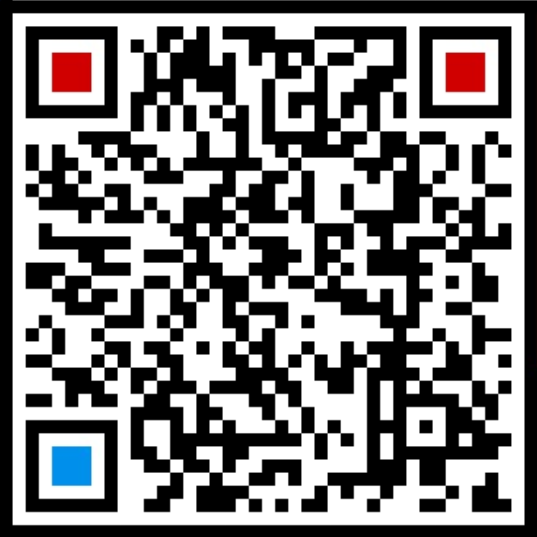
\includegraphics[width=2.2cm]{images/wx_qrcode.png}}; 
\end{tikzpicture}


\makecvtitle % Print the CV title

%----------------------------------------------------------------------------------------
%	EDUCATION SECTION
%----------------------------------------------------------------------------------------

\ifEducationSection

\ifChinese

\section{教育背景}

\cventry{2010.9--2018.1}{清华大学}{}{}{}{\normalsize 理学博士,数学}

\cventry{2006.8--2010.6}{清华大学}{}{}{}{\normalsize 理学学士,数学物理基础科学班}

\ifHighSchool
\cventry{2002.9--2006.6}{萍乡中学}{}{}{}{}
\fi

\else  % else of \ifChinese

\section{Education}

\cventry{2010.9--2018.1}{Tsinghua University}{}{}{}{\normalsize {\bfseries Doctor} of Philosophy, \textit{Mathematics}}

\cventry{2006.8--2010.6}{Tsinghua University}{}{}{}{\normalsize {\bfseries Bachelor} of Science, \textit{Mathematics and Physics}}

\fi  % fi of \ifChinese

\fi  % fi of \ifEducationSection


%----------------------------------------------------------------------------------------
%	AWARDS SECTION
%----------------------------------------------------------------------------------------

\ifAwardsSection

\ifChinese

\section{获得奖励}

% \cventry{April 2015 --
% April 2017}{Certified LabVIEW Associate Developer}{\textsc{National Instruments}}{}{}{}

\else  % else of \ifChinese

\section{Certifications}

% \cventry{April 2015 --
% April 2017}{Certified LabVIEW Associate Developer}{\textsc{National Instruments}}{}{}{}

\fi  % fi of \ifChinese

\fi  % fi of \ifAwardsSection


%----------------------------------------------------------------------------------------
%	RESEARCH INTEREST SECTION
%----------------------------------------------------------------------------------------

\ifResearchInterestSection

\ifChinese

\section{研究领域}

\cvitem{}{
\textbf{机器学习,深度学习,最优化理论与应用}
\newline
数论,代数几何,表示论 ,密码学,模式识别,信号处理
}

\else  % else of \ifChinese

\section{Research Interests}

\cvitem{}{\textbf{Federated Learning, Deep Learning, Mathematical Optimization} - Theory and Applications
\newline
Number Theory, Arithmetic Geometry, Representation Theory, Cryptography, Pattern Recognition
}

\fi  % fi of \ifChinese

\fi  % fi of \ifResearchInterestSection


%----------------------------------------------------------------------------------------
%	RESEARCH EXPERIENCE SECTION
%----------------------------------------------------------------------------------------

\ifResearchExperienceSection

\ifChinese

\section{研究经历}

\cventry{2021.3
至今}{Federated Learning, Large-Scale Non-Convex Optimization}{\newline 合作导师:韩德仁教授}{北京航空航天大学}{}{}

\cventry{2019.1 --
2021.1}{Cognitive Computing for Precision Health}{\newline 合作导师:喻文健副教授,吴元清博士}{清华大学,京东健康医疗创新研发部}{}{}

\cventry{2017.3 --
2018.1}{Counting Multiplicities in a Hypersurface over Number Fields}{\newline 合作者:刘春晖博士}{Universit\'{e} Paris Diderot,法国}{}{}

\cventry{2016.5 --
2017.3}{Characters of the General Linear Supergroups}{\newline 指导教师:张贺春教授}{清华大学}{}{}

\cventry{2014.1 --
2015.6}{Computation of Modular Units}{\newline 指导教师:印林生教授}{清华大学}{}{}

\cventry{2013.1 --
2013.7}{N\'{e}ron Models of Semi-Abelian Varieties}{\newline 访问学者}{\emph{指导教师:刘青教授}}{Universit\'{e} Bordeaux 1,法国}{}

\cventry{2012.1 --
2013.12}{Galois Representation and Modular Forms}{\newline 指导教师:印林生教授}{清华大学}{}{}

\cventry{2011.1 --
2012.12}{Elliptic-Curve Cryptography}{\newline 指导教师:印林生教授}{清华大学}{}{}

\else  % else of \ifChinese

\section{Research Experience}

\cventry{Jan. 2021 -- Current}{Federated Learning, Large-Scale Non-Convex Optimization}{\newline School of Mathematical Sciences}{Beihang University}{}{}

\cventry{Jan. 2019 -- Jan. 2021}{Cognitive Computing for Precision Health}{\newline Department of Computer Science and Technology}{Tsinghua University}{}{}

\cventry{Mar. 2017 -- Jan. 2018}{Counting Multiplicities in a Hypersurface over Number Fields}{\newline Co-author with Dr. Chunhui Liu}{Universit\'{e} Paris Diderot}{}{}

\cventry{May 2016 -- Mar. 2017}{Characters of the General Linear Supergroups}{\newline Research team of Prof. Hechun Zhang}{Department of Mathematical Sciences}{Tsinghua University}{}

\cventry{Jan. 2014 -- June 2015}{Computation of Modular Units}{\newline Research team of Prof. Linsheng Yin}{Department of Mathematical Sciences}{Tsinghua University}{}

\cventry{Jan. 2013 -- June 2013}{N\'{e}ron Models of Semi-Abelian Varieties}{\newline Visiting Scholar}{Universit\'{e} Bordeaux 1}{France}{}

\cventry{Jan. 2012 -- Dec. 2013}{Galois Representation and Modular Forms}{\newline Research team of Prof. Linsheng Yin}{Department of Mathematical Sciences}{Tsinghua University}{}

\cventry{Jan. 2011 -- Dec. 2012}{Elliptic-Curve Cryptography}{\newline Research team of Prof. Linsheng Yin}{Tsinghua University}{}{}

\fi  % fi of \ifChinese

\fi  % fi of \ifResearchExperienceSection


%----------------------------------------------------------------------------------------
%	WORK EXPERIENCE SECTION
%----------------------------------------------------------------------------------------

\ifWorkExperienceSection

\ifChinese

\section{创业与工作经历}

\cventry{2021.3 至今}{北京航空航天大学博士后}{}{}{}{联邦学习中的优化算法以及在医疗中的应用;深度学习在医学图像、信号处理中的应用。}

\cventry{2018.10 --
2021.1}{京东健康医疗创新研发部算法工程师、企业博士后}{}{}{}{采用传统信号处理,模式识别,结合机器学习深度学习等多种工具,与京东健康医疗创新研发部同事合作,分别搭建了3个完整的智慧医疗系统,包括连续血糖监护分析平台,心电监护分析平台,以及中医望诊平台。}

\cventry{2014.10 --
2016.9}{与别人合伙创立\textsc{Houyi Tech., Inc.},并担任兼职算法开发人员}{}{}{}{采用小面积传感器在嵌入式的 ARM STM32 嵌入式芯片上实现了指纹认证系统(软件著作权登记号2015SR079424),并在消费电子以及公证处等多个场景落地。}

\else  % else of \ifChinese

\section{Entrepreneurial and Work Experience}

\cventry{2021.3 --
Current}{\textsc{Beihang University}}{Postdoctoral Fellow}{}{}{Optimization algorithms in Federated Learning and applications in Healthcare; Applications of deep learning in medical image and signal processing.}

\cventry{2018.10 --
2021.1}{\textsc{JD Health International Inc.}}{Algorithm Engineer and Corporate Postdoctoral Fellow}{}{}{Pattern recognition, machine learning and deep learning for medical image and signal processing; Design and implement smart medical systems: continuous blood glucose monitoring and analysis platform, ECG monitoring analysis platform, the TCM observation and diagnosis platform.}

\cventry{2014.10 --
2016.9}{\textsc{Houyi Tech. Inc.}}{Co-founder and Algorithm Engineer}{}{}{Embedded Implementation of Fingerprint Recognition Systems on ARM STM32 platforms.}

\fi  % fi of \ifChinese

\fi  % fi of \ifWorkExperienceSection


%----------------------------------------------------------------------------------------
%	PUBLICATIONS SECTION
%----------------------------------------------------------------------------------------

\ifPublicationsSection

\ifChinese

\nocite{phdthesis-zh,wen_liu,Kang_2022_cinc2021_iop,torch_ecg_paper,Wen_cpsc2021,wen_cinc2021,qi2021kemre,af_detection,acne_detection}
\printbibliography[title={发表文章}]

\else  % else of \ifChinese

\nocite{phdthesis-en,wen_liu,Kang_2022_cinc2021_iop,torch_ecg_paper,Wen_cpsc2021,wen_cinc2021,qi2021kemre,af_detection,acne_detection}
\printbibliography[title={Publications}]

\fi  % fi of \ifChinese

\fi  % fi of \ifPublicationsSection


%----------------------------------------------------------------------------------------
%	Ph.D. SECTION
%----------------------------------------------------------------------------------------

\ifPhdThesisSection

\ifChinese

\section{博士论文}

\cvitem{题目}{\bfseries 定义在数域上的超曲面的重数计数问题}
\cvitem{导师}{{\bfseries 张贺春} 教授}
\cvitem{评审人}{唐舜,徐飞(首都师范大学),\newline
王崧(中国科学院晨兴数学中心),\newline
姚家燕(清华大学)}
\cvitem{答辩委员会}{徐飞({\bfseries 主席},首都师范大学),\newline
郑维喆(中国科学院晨兴数学中心),\newline
姚家燕,朱斌,邓邦明(清华大学)}
\cvitem{论文简介}{考虑定义在数域上的射影超曲面,可以通过局部 Hilbert-Samuel 函数定义其上点的重数。取定一个计数函数,考虑在这个射影超曲面上代数点的重数的计数问题:即对超曲面上,高度不超过定值,定义域相对于基域的扩张次数等于一个定值的所有代数点,用取定的计数函数作用在这些点的重数上,求和。论文对这个问题给出了一个上界估计,这个上界将会与射影超曲面的次数,奇点集的维数,高度的上界,以及相应域扩张次数有关。这个估计可以在某种程度上衡量射影超曲面的奇点集的复杂程度。}

\else  % else of \ifChinese

\section{Ph.D. Thesis}

\cvitem{Title}{\emph{Counting Multiplicities in a Hypersurface over Number Fields}}
\cvitem{Supervisor}{Professor {\bfseries Hechun ZHANG}}
\cvitem{Reviewers}{Shun TANG, Fei XU (Capital Normal University),\newline Song WANG (Chinese Academy of Sciences),\newline Jiayan YAO (Tsinghua University)}
\cvitem{Committee Members}{Fei XU ({\bfseries Chair}, Capital Normal University),\newline Weizhe ZHENG (Chinese Academy of Sciences),\newline Jiayan YAO, Bin ZHU, Bangming DENG (Tsinghua University)}
\cvitem{Description}{Fix a counting function of multiplicities of algebraic points in a projective hypersurface over a number field, and take the sum over all algebraic points of bounded height and fixed degree. An upper bound for the sum with respect to this counting function is given in terms of the degree of the hypersurface, the dimension of the singular locus, the upper bounds of height, and the degree of the field of definition. This upper bound describes the complexity of this hypersurface's singular locus to some extent.}

\fi  % fi of \ifChinese

\fi  % fi of \ifPhdThesisSection


%----------------------------------------------------------------------------------------
%	INVITED TALKS SECTION
%----------------------------------------------------------------------------------------

\ifInvitedTalksSection

\ifChinese

\section{受邀报告}

\cventry{2022.9}{The 49th Computing in Cardiology Conference}{\newline \textsc{题目:Searching for Effective Neural Network Architectures for Heart Murmur Detection from Phonocardiogram}}{\newline Poster}{Online (offline at Tampere, Finland)}{}

\cventry{2021.11}{The 10th International Conference on Biomedical Engineering and Biotechnology (ICBEB 2021)}{\newline \textsc{题目:Accurate Paroxysmal Atrial Fibrillation Events
Detection using Deep Neural Networks}}{\newline Oral}{Online}{}

\cventry{2021.9}{The 48th Computing in Cardiology Conference}{\newline \textsc{题目:Hybrid Arrhythmia Detection on Varying-Dimensional ECG: Combining Deep Neural Networks and Clinical Rules}}{\newline Poster}{Online (offline at Brno, Czech Republic)}{}

\cventry{2017.9}{Intercity Seminar on Arakelov Theory, the 2017 Session in Beijing}{\newline \textsc{题目:Counting Multiplicities in a Hypersurface over Number Fields}}{\newline 首都师范大学}{北京}{}

\cventry{2017.4}{清华大学博士生论坛}{\newline \textsc{题目:Characters of the General Linear Supergroups}}{\newline 三堡学术基地}{北京}{}

\else  % else of \ifChinese

\section{Invited Talks}

\cventry{2022.9}{The 49th Computing in Cardiology Conference}{\newline \textsc{Title: Searching for Effective Neural Network Architectures for Heart Murmur Detection from Phonocardiogram}}{\newline Poster}{Online (offline at Tampere, Finland)}{}

\cventry{Nov. 2021}{The 10th International Conference on Biomedical Engineering and Biotechnology (ICBEB 2021)}{\newline \textsc{Title: Accurate Paroxysmal Atrial Fibrillation Events
Detection using Deep Neural Networks}}{\newline Oral}{Online}{}

\cventry{Sept. 2021}{The 48th Computing in Cardiology Conference}{\newline \textsc{Title: Hybrid Arrhythmia Detection on Varying-Dimensional ECG: Combining Deep Neural Networks and Clinical Rules}}{\newline Poster}{Online (offline at Brno, Czech Republic)}{}

\cventry{Sept. 2017}{Intercity Seminar on Arakelov Theory, the 2017 Session in Beijing}{\newline \textsc{Title: Counting Multiplicities in a Hypersurface over Number Fields}}{\newline Capital Normal University}{Beijing}{}

\cventry{Apr. 2017}{Forum of Ph.D. Candidates organised by Tsinghua University}{\newline \textsc{Title: Characters of the General Linear Supergroups}}{\newline Sanbao Academic Base}{Beijing}{}

\fi  % fi of \ifChinese

\fi  % fi of \ifInvitedTalksSection


%----------------------------------------------------------------------------------------
% TEACHING EXPERIENCE SECTION
%----------------------------------------------------------------------------------------

\ifTeachingSection

\renewcommand{\listitemsymbol}{-~} % Changes the symbol used for lists

\ifChinese

\section{助教工作}

\cvlistdoubleitem{高等代数}{微积分}
\cvlistdoubleitem{代数数论}{抽象代数}
% \cvlistdoubleitem{高等代数与几何}{}

\else  % else of \ifChinese

\section{Teaching Assistant}

\cvlistdoubleitem{Calculus}{Advanced Calculus}
\cvlistdoubleitem{Linear Algebra}{Advanced Algebra}
\cvlistdoubleitem{Algebraic Number Theory}{Abstract Algebra}
% \cvlistdoubleitem{Advanced Algebra and Geometry}{}

\fi  % fi of \ifChinese

\fi  % fi of \ifTeachingSection


%----------------------------------------------------------------------------------------
% Miscellaneous SECTION
%----------------------------------------------------------------------------------------

\ifMiscSection

\ifChinese

\section{其他经历}

\cventry{Jul. 2012 --
Aug. 2012}{Dongfang Electric Corporation}{}{Guangzhou}{}{Research and technological development of information security of the enterprise.}

\cventry{2020.11}{3rd China Physiological Signal Challenge 2020 (CPSC2020) 竞赛项目 SPBerr 第三名}{}{}{}{}{}

\cventry{2014.9 --
2015.12}{课程助教}{\href{http://www.xuetangx.com/}{学堂在线}}{}{}{作为清华大学数学系马辉教授所教授的《线性代数1》与《线性代数2》的学堂在线MOOC课程的助教,协助其制作PPT课件,并维护课程论坛。}

\cventry{2014.8 --
2014.10}{China-Korea Joint Seminar on Number Theory}{}{海南三亚}{}{协助印林生教授组织会议。}

\cventry{2014.10 --
2015.12}{兼职算法开发人员}{\textsc{Houyi Tech., Inc.}}{}{}{与别人合作,在 ARM STM32 嵌入式芯片上实现了指纹识别等功能(软件著作权登记号2015SR079424),并在多个应用场景落地。}

\else  % else of \ifChinese

\section{Miscellaneous}

\cventry{Nov. 2020}{3rd place in SPBerr in the 3rd China Physiological Signal Challenge 2020 (CPSC2020)}{}{}{}{}{}

\cventry{Jul. 2012 --
Aug. 2012}{Dongfang Electric Corporation}{}{Guangzhou}{}{Research and technological development of information security of the enterprise.}

\cventry{Oct. 2014 --
Dec. 2015}{Algorithm Developer}{\textsc{Houyi Tech., Inc.}}{Beijing}{}{Implementing fingerprint identification algorithm (system) on ARM STM 32 embedded chip.}

\cventry{Aug. 2014 --
Oct. 2014}{China-Korea Joint Seminar on Number Theory}{}{Sanya}{}{Assisting Prof. Linsheng Yin in organizing the conference}

\cventry{Sept. 2014 --
Dec. 2015}{Teaching Assistant}{\href{http://www.xuetangx.com/}{xuetangx.com}}{}{}{Assisting Prof. Hui Ma of the Math department in Tsinghua University in preparing lecture ppt, and maintaining the course forum}

\fi  % fi of \ifChinese

\fi  % fi of \ifMiscSection


% ----------------------------------------------------------------------------------------
% 	LANGUAGES SECTION
% ----------------------------------------------------------------------------------------

\ifLanguageSection

\ifChinese

\section{语言能力}

% \cvitemwithcomment{Chinese}{Native Language}{}
\cvitemwithcomment{英语}{流利}{清华英语水平2, CET-6, PETS5}
\cvitemwithcomment{法语}{一般}{}

\else  % else of \ifChinese

\section{Languages}

\cvitemwithcomment{Chinese}{Native Language}{}
\cvitemwithcomment{English}{Fluent}{Tsinghua Level 2, CET-6, PETS5}
\cvitemwithcomment{French}{Intermediate}{}

\fi  % fi of \ifChinese

\fi  % fi of \ifLanguageSection


%----------------------------------------------------------------------------------------
%	Skills and Open source community SECTION
%----------------------------------------------------------------------------------------

\ifSkillsAndOscSection

\ifChinese

\section{其他技能以及开源社区贡献}

\cvitem{编程语言}{\textsc{Python, R, Matlab, Mathematica, C, C++, LaTeX}}
% \cvitem{驾照}{C1}

\else  % else of \ifChinese

\section{Skills \& Open Source Community Contributions}

% \cvitem{Programming}{\textsc{Python, R, Matlab, Mathematica, C, C++, LaTeX}}

\fi  % fi of \ifChinese


\cvitem{Repositories}{
\hspace{-0.2em}-~~\href{https://github.com/DeepPSP/torch_ecg}{https://github.com/DeepPSP/torch\_ecg}\newline
% -~~\href{https://github.com/DeepPSP/bib_lookup}{https://github.com/DeepPSP/bib\_lookup}\newline
-~~\href{https://github.com/DeepPSP/DBCI}{https://github.com/DeepPSP/DBCI}\newline
-~~\href{https://github.com/wenh06/fl_seminar}{https://github.com/wenh06/fl\_seminar} \newline
-~~\href{https://gitee.com/wenh06/buaa-advanced-algebra-2021}{https://gitee.com/wenh06/buaa-advanced-algebra-2021}\newline
-~~\href{https://git.openi.org.cn/Numbda/AI-Testing}{https://git.openi.org.cn/Numbda/AI-Testing} (Docs: \href{https://numbda.cs.tsinghua.edu.cn/AI-Testing}{https://numbda.cs.tsinghua.edu.cn/AI-Testing})
}
\cvitem{Contributor}{
\href{https://github.com/pytorch/pytorch}{PyTorch}, \href{https://github.com/QData/TextAttack}{TextAttack}, \href{https://github.com/Tianxiaomo/pytorch-YOLOv4}{pytorch-YOLOv4}
}

\fi  % fi of \ifSkillsAndOscSection


% ----------------------------------------------------------------------------------------
% 	PERSONAL INTERESTS SECTION
% ----------------------------------------------------------------------------------------

\ifInterestsSection

\renewcommand{\listitemsymbol}{-~} % Changes the symbol used for lists

\ifChinese

\section{兴趣爱好}
% \cvlistdoubleitem{Piano}{}
\cvlistitem{足球}
\cvlistitem{阅读}

\else  % else of \ifChinese

\section{Interests}
% \cvlistdoubleitem{Piano}{}
\cvlistitem{Football}
\cvlistitem{Reading}

\fi  % fi of \ifChinese

\fi  % fi of \ifInterestsSection


%----------------------------------------------------------------------------------------
%	LIST OF REFERENCES
%----------------------------------------------------------------------------------------

\ifListReferences

\section{References}

\cvdoublecolumn{
    \cvreference{Hechun ZHANG}
    {}
    {Department of Mathematical Sciences}
    {Tsinghua University}
    {Beijing, China}
    {\href{http://faculty.math.tsinghua.edu.cn/~hzhang/}{http://faculty.math.tsinghua.edu.cn/~hzhang/}}
    {hzhang@math.tsinghua.edu.cn}
    {}
    {}
    }
    % {\cvreference{Jing YANG}
    % {}
    % {Department of Mathematical Sciences}
    % {Tsinghua University}
    % {Beijing, China}
    % {}
    % {jingyang@math.tsinghua.edu.cn}
    % {}
    % {}
    % }
    {\cvreference{Wenjian YU}
    {}
    {Department of Computer Science and Technology}
    {Tsinghua University}
    {Beijing, China}
    {\href{http://numbda.cs.tsinghua.edu.cn/~yuwj/}{http://numbda.cs.tsinghua.edu.cn/~yuwj/}}
    {yu-wj@tsinghua.edu.cn}
    {}
    {}
    }

\fi  % fi of \ifListReferences


%----------------------------------------------------------------------------------------
%	COVER LETTER
%----------------------------------------------------------------------------------------

\ifCoverLetter

\clearpage

\ifChinese

\recipient{HR Department}{Corporation\\123 Pleasant Lane\\12345 City, State} % Letter recipient
\date{\today} % Letter date
\opening{Dear Sir or Madam,} % Opening greeting
\closing{Sincerely yours,} % Closing phrase
\enclosure[Attached]{curriculum vit\ae{}} % List of enclosed documents

\makelettertitle % Print letter title

\zhlipsum[1-3] % Dummy text

\makeletterclosing % Print letter signature

\else  % else of \ifChinese

\recipient{HR Department}{Corporation\\123 Pleasant Lane\\12345 City, State} % Letter recipient
\date{\today} % Letter date
\opening{Dear Sir or Madam,} % Opening greeting
\closing{Sincerely yours,} % Closing phrase
\enclosure[Attached]{curriculum vit\ae{}} % List of enclosed documents

\makelettertitle % Print letter title

\lipsum[1-3] % Dummy text

\makeletterclosing % Print letter signature

\fi  % fi of \ifChinese

\fi  % fi of \ifCoverLetter


%----------------------------------------------------------------------------------------
% TEACHING STATEMENT
%----------------------------------------------------------------------------------------

\ifTeachingStatement

\ifChinese



\else



\fi  % fi of \ifChinese

\fi  % fi of \ifCoverLetter


%----------------------------------------------------------------------------------------
% RESEARCH STATEMENT
%----------------------------------------------------------------------------------------

\ifResearchStatement

\ifChinese


\else


\fi  % fi of \ifChinese

\fi  % fi of \ifCoverLetter



%------- End of the contents ------------------------------------------------------------



%-------------------------------------------------------

\end{document}
